% File SDSS2020_SampleExtendedAbstract.tex
\documentclass[10pt]{article}
\usepackage{sdss2020} % Uses Times Roman font (either newtx or times package)
\usepackage{url}
\usepackage{latexsym}
\usepackage{amsmath, amsthm, amsfonts}
\usepackage{algorithm, algorithmic}
\usepackage{graphicx}
\usepackage[capitalise]{cleveref}
\usepackage{caption}

\usepackage[dvipsnames]{xcolor} % colors
\newcommand{\mh}[1]{{\textcolor{blue}{#1}}}
\newcommand{\svp}[1]{{\textcolor{RedOrange}{#1}}}

% %% Author information
% \author{Muxin Hua\\
%   Statistics Department\\ \\
% {\tt mhua2@huskers.unl.edu}\\\And Susan Vanderplas\\
%   Statistics Department\\ \\
% {\tt susan.vanderplas@unl.edu}\\}
%
\title{Automatic Acquisition and Identification of Footwear Class
Characteristics}
\setlength\titlebox{2.5cm}
\date{}

\begin{document}
\maketitle
\begin{abstract}
% The identification of footwear is routinely performed in the field of forensic _science_.
% _Good attempt at a lead-in, but let's try to make it a bit more specific - the problem isn't that footwear identification is important, but that we're trying to make evaluation of that evidence more quantitative_
\svp{Forensic footwear examination is currently subjective, with no way to quantify the uniqueness of the print's features relative to the population footwear characteristics.
% The common methods of identifying are gathering data with surveillance devices and assessing with huge amount of human labor.
%_Good, this is identifying the impact of the work you've done_
In the past, gathering any population data on footwear has required individually collecting prints from individuals in public, and then manually identifying characteristics from those prints.
% The emergence of convolution network inspires a new approach allows for differentiating shoe from background, locating regions of interest, and labeling these regions of interest with appropriate features.
% _The network didn't just emerge - you built it! It didn't show up from the ether!_
In this paper, we present a convolutional neural network which identifies and classifies characteristics of shoe prints in human-friendly terms.
When paired with a newly developed scanner which can collect prints from people walking across it on public paths, these innovations represent a significant step forward in laying a foundation for quantitative evaluation of forensic footwear evidence.}

\end{abstract}


\section{Introduction}
% Explain what the real world problem is
\svp{Forensic investigations frequently turn up shoe prints which are informative but not sufficiently detailed to identify a single individual. The features provided by these prints are known as \emph{class characteristics}: they may be shared by many shoes of the same make and model, but are useful for narrowing down a subject pool and providing some association between a suspect and the scene \cite{bodziakFootwearImpressionEvidence2000}.}
% Figure: examples of class characteristics

% Triangle Circle Star
% Include a second set of pictures showing another classification metric (SoleMate) so that we can discuss the differences between the two.

%Explain the connection between the real world problem and our solution
\svp{
When assessing the worth of class characteristic evidence, it is helpful to know more about the distribution of class characteristics in the local population \cite{grossVariabilitySignificanceClass2013}.
These characteristics are likely to have high geographic variability (because of weather, population composition, etc.), so this data must be gathered and compared at a local level.
% To statistically calculate the random match probability of footwear, we need shoe data from a given population. It has been an impossible task to collect all the shoe data from a population given the data volume and variety.
Collection and processing of footwear data has historically required large amounts of human labor, which has made collection of the necessary population data infeasible for law enforcement agencies.
We have collaborated with engineers to develop a shoe scanner capable of gathering this data automatically, but the data still needs to be processed to identify relevant features.
% In this research, we adopt a viable solution: collecting data with a scanner and automatically classifying image with transfer learning on Faster Region-based Convolution Neural Network (Faster R-CNN).
In this paper, we describe a faster, region-based convolutional neural network (R-CNN) \cite{girshickFastRCNN2015} which identifes areas of the shoe sole with relevant class characteristic features and applies human-readable labels to those features.
Previous approaches to shoeprint classification and retrieval used CNN features directly \cite{zhangAdaptingConvolutionalNeural2017}, but these features are not describable or useable by forensic examiners.
The additional step of using human-friendly labels introduces additional complexities to the problem of class characteristic identification, but also makes a model which is more useful for the task of assisting forensic examiners with quantifying the significance, weight, and importance of the evidence they present in court.
We hope that the combination of the scanner and the computer vision model will lay the foundation for more effective and quantitative characterization of the relevance and weight of footwear evidence.}



\section{Methods}


\subsection{Computer Vision Models}
% Provide a brief overview of classification vs. identification, the differences between CNN and RCNN models, and why RCNN is ideal for this use case.
% Show the "what we want" picture with a real shoe print and several bounding boxes labeled.
\svp{In the past decade, the field of computer vision has exploded, with models capable of identifying subtle differences between visually similar animals, vehicles, and plants in the natural world.
Most of these models utilize convolutional neural networks, which encode features in a local neighborhood around each pixel in a photograph, and then have structure which allows the network to encode some higher-level feature information through relationships between lower-level features.
% Faster R-CNN has the ability of extracting and identifying features and output a set of interesting regions with labels of classes and corresponding predictive scores.
We have previously used VGG16 to identify class characteristic features, but it is an older network that requires images of a specific size; this necessitated tiling a shoe sole image into smaller regions and making predictions on each sub-image before reassembling the shoe sole and integrating the predictions.
In this paper, we explore the use of the Faster R-CNN model, which can work with the full shoe sole image.
This model identifies regions with interesting features and then labels them with probabilities representing each feature in the training data.
}

% To serve our purpose of identifying features in image_s_, we implement transfer learning on Faster R-CNN to detect shoe tread features.
\svp{
Training a convolutional neural network from scratch requires a large amount of computational resources and a considerable amount of training data.
While we have the ability to acquire previously incomprehensible quantities of images from the shoe scanner our engineering collaborators developed, there is still at least an order of magnitude less data available than would be required to train a network from scratch.
}



\subsection{Transfer Learning}
Transfer Learning is a technique \svp{which} uses weights from pretrained models to solve a new problem.
Pretrained \svp{computer vision} models, like Resnet101 \svp{and} VGG-16 \svp{are developed} on massive \svp{amounts of labeled photographic} data\svp{, which allows them to successfully differentiate between a wide variety of naturally occurring objects}.
\svp{Many of the feature detectors which allow these networks to function so well are also relevant to the detection of geometric images on shoe soles.}
\svp{Leveraging} these models \svp{allows us to make more efficient use of the data we have} while achieving lower error rates.

\svp{
In this paper, we describe the process of implementing single-stage transfer learning for shoe images.
While we do have a shoe scanner which is collecting real-world data, we have only been collecting that data for a relatively short period of time, and it has not yet been manually annotated.
For the first stage of this training process, we use labeled photographs of shoe soles taken from online retailers: this allows us to focus primarily on the identification of geometric features using human-friendly class labels.
While geometric feature identification sounds simple, in practice it is extremely challenging, as discussed in \Cref{sec:classification-scheme}.}

% We start with training shoe sole pictures from Zappos, a shoe retailer website provides clear, nice shoe sole images perfect for training. This process emphasizes the feature detectors that work with shoe tread patterns. To further robust the network, we will train the model on scanner data, which has degradation image quality.  % I wrote the paragraphs above and below this before I got to that paragraph :)  Great minds think alike.

\svp{Once we have a network which emphasizes feature detectors useful for identifying class characteristics in "clean" images, we conduct a second stage of transfer learning which will allow the model to cope with degraded real-world images, which may be obscured with dirt or have suboptimal lighting.}

\subsection{Class Characteristic Labels}\label{sec:classification-scheme}
\svp{
Perceptually, we do not usually have much trouble differentiating between a circle and a square - circles are round, squares have straight lines of equal length that meet in equal angles.
This simple observation becomes much more complicated when applied to creating labeling criteria for shoe sole design patterns: not all shoe sole materials accommodate sharp corners, shoes wear down over time, and some shapes are simply ambiguous, as shown in  \Cref{fig:dc-shoe}.
In addition, while humans can use context to clarify some ambiguous features (such as the difference between a dot on an 'i' and a circle), computer vision models typically do not have this ability.
An example of this phenomenon is provided in \Cref{fig:adidas}.
Mitigating this problem requires a combination of careful labeling of training data (to provide information to the computer that is at the level that the models can use) and identification of a sufficiently distinct set of class characteristics.
A distinct set of class characteristics is essential to reduce cross-classification errors which stem from the data rather than the model's discriminatory capabilities.
In this paper, we discuss the impact of different sets of class characteristic labels on R-CNN model performance, and consider what misclassification looks like with contextual information (or lack thereof) for forensic examiners as well as computer vision models.
}

% Although we have determined the footwear shapes, it’s still difficult to annotate the images. Unlike other image classifications, geometric features of footwear are artificial and difficult to annotate. For example, in this image from a DC shoe, there are repeating patterns of a shape, but this shape doesn’t strictly fall into any of the categories. It’s a mixture of circle, quadrilateral and text of “D” and “C”. Th ambiguity of feature has been a huge challenge in this study.

\begin{figure}
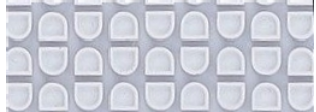
\includegraphics[width=\linewidth]{dc_circle_quad.png}
\caption{Some common shapes on shoe soles blur the lines between two categories. This pattern, which is frequently found on DC shoes, is halfway between a circle and a square, and could reasonably be classified as either shape.}\label{fig:dc-shoe}
\end{figure}

\begin{minipage}{.4\linewidth}
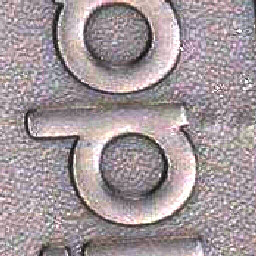
\includegraphics[width=\linewidth]{adidas-test.jpg}
\end{minipage}\hfill\begin{minipage}{.49\linewidth}
\captionof{figure}{Without context, some shoe features appear to be one category, while a human annotating the full image would label this another category. Here, the inside of the "a" and "d" in Adidas are perfect circ es.\label{fig:adidas}}
\end{minipage}


\section{Results}
% In this work, we described the process of training and evaluating each stage of the model. We are looking forward to being able to identify the features with the accuracy of “nice” and “scanner” models.  (Maybe show a picture of our prediction if I can complete the code)
\svp{
In this paper, we describe the process of fitting a faster R-CNN model to annotated shoe data using geometric descriptors as well as a system for class characteristic labeling used by forensic examiners.
We assess the difference that the classification scheme makes to the model fitting process as well as numerical measures of the models' utility and how these measures hold up under the unique constraints of labeling footwear tread pattern features.
We also explore the accuracy of the initial stage of the transfer learning model process when the model is used to directly predict features of images captured from the shoe scanner directly.
}


\section{Discussion }
% Interesting points for discussion -
%   - If the model identifies something that is present but wasn't labeled, is that an error?
%   - Examiners don't care about the model's ability to use context or that it tends to assign multiple labels - they work in a space where there are many different descriptors that sometimes overlap.
This work provides the ability to study the distribution of class characteristics in footwear.
Utilizing the Faster R-CNN and the weights of pretrained models,
%our task can be implemented efficiently.
\svp{we can use a smaller set of labeled data to identify class characteristics using human-friendly labels, leveraging these computer vision models' abilities on a niche set of training labels.}

\svp{One interesting facet of this problem is the effect of contextual information on the labeling process.
Human examiners often have to work with incomplete prints, which may not have the contextual information useful for differentiating between a circle and the letter 'o'; as a result, while the computer vision models often confuse the two features (which are labeled differently), human examiners would not consider this misclassification to be an error.
In statistical and machine learning problems, it is less common to have misclassifications which are ambiguously errors (or not).
We discuss the implications of this problem for interpreting the results of our model and consider how human labels impact the underlying approach to using computer vision techniques in forensics.
}


\bibliographystyle{sdss2020} % Please do not change the bibliography style
\bibliography{references}


\end{document}
